\documentclass{beamer}\usepackage{graphicx, color}
%% maxwidth is the original width if it is less than linewidth
%% otherwise use linewidth (to make sure the graphics do not exceed the margin)
\makeatletter
\def\maxwidth{ %
  \ifdim\Gin@nat@width>\linewidth
    \linewidth
  \else
    \Gin@nat@width
  \fi
}
\makeatother

\IfFileExists{upquote.sty}{\usepackage{upquote}}{}
\definecolor{fgcolor}{rgb}{0.2, 0.2, 0.2}
\newcommand{\hlnumber}[1]{\textcolor[rgb]{0,0,0}{#1}}%
\newcommand{\hlfunctioncall}[1]{\textcolor[rgb]{0.501960784313725,0,0.329411764705882}{\textbf{#1}}}%
\newcommand{\hlstring}[1]{\textcolor[rgb]{0.6,0.6,1}{#1}}%
\newcommand{\hlkeyword}[1]{\textcolor[rgb]{0,0,0}{\textbf{#1}}}%
\newcommand{\hlargument}[1]{\textcolor[rgb]{0.690196078431373,0.250980392156863,0.0196078431372549}{#1}}%
\newcommand{\hlcomment}[1]{\textcolor[rgb]{0.180392156862745,0.6,0.341176470588235}{#1}}%
\newcommand{\hlroxygencomment}[1]{\textcolor[rgb]{0.43921568627451,0.47843137254902,0.701960784313725}{#1}}%
\newcommand{\hlformalargs}[1]{\textcolor[rgb]{0.690196078431373,0.250980392156863,0.0196078431372549}{#1}}%
\newcommand{\hleqformalargs}[1]{\textcolor[rgb]{0.690196078431373,0.250980392156863,0.0196078431372549}{#1}}%
\newcommand{\hlassignement}[1]{\textcolor[rgb]{0,0,0}{\textbf{#1}}}%
\newcommand{\hlpackage}[1]{\textcolor[rgb]{0.588235294117647,0.709803921568627,0.145098039215686}{#1}}%
\newcommand{\hlslot}[1]{\textit{#1}}%
\newcommand{\hlsymbol}[1]{\textcolor[rgb]{0,0,0}{#1}}%
\newcommand{\hlprompt}[1]{\textcolor[rgb]{0.2,0.2,0.2}{#1}}%

\usepackage{framed}
\makeatletter
\newenvironment{kframe}{%
 \def\at@end@of@kframe{}%
 \ifinner\ifhmode%
  \def\at@end@of@kframe{\end{minipage}}%
  \begin{minipage}{\columnwidth}%
 \fi\fi%
 \def\FrameCommand##1{\hskip\@totalleftmargin \hskip-\fboxsep
 \colorbox{shadecolor}{##1}\hskip-\fboxsep
     % There is no \\@totalrightmargin, so:
     \hskip-\linewidth \hskip-\@totalleftmargin \hskip\columnwidth}%
 \MakeFramed {\advance\hsize-\width
   \@totalleftmargin\z@ \linewidth\hsize
   \@setminipage}}%
 {\par\unskip\endMakeFramed%
 \at@end@of@kframe}
\makeatother

\definecolor{shadecolor}{rgb}{.97, .97, .97}
\definecolor{messagecolor}{rgb}{0, 0, 0}
\definecolor{warningcolor}{rgb}{1, 0, 1}
\definecolor{errorcolor}{rgb}{1, 0, 0}
\newenvironment{knitrout}{}{} % an empty environment to be redefined in TeX

\usepackage{alltt}
\usetheme{Stats}
\setbeamercovered{transparent}
\usepackage{color}
\usepackage{hyperref}
  \hypersetup{
  	colorlinks=true
		linkcolor=black
		}
\usepackage{url}
\usepackage{graphics}
\usepackage{tikz}
\usepackage{booktabs}





%%%%%%%%%%%%%%%%%%%%%%%%%%%%%%%% Title Slide %%%%%%%%%%%%%%%%%%%%%%%%%%
\title[Lecture 2]{Intro to Social Science Data Analysis \\[1cm] Lecture 2: Types of Data}
\author[]{
    \href{mailto:gandrud@yonsei.ac.kr}{Christopher Gandrud}
}
\date{\today}


\begin{document}



\frame{\titlepage}

\section[Outline]{}
\frame{\tableofcontents}

\section{Review}
\frame{
  \frametitle{Open Intro Textbook}
  They recently released a second edition of the Open Intro book. \\[0.5cm]
  For now, {\bf{continue to use the first edition}}.
}

\frame{
	\frametitle{Recap}
  Last week we: \\[0.5cm]
  \begin{itemize}
    \item<1-> {\bf{Installed}} R, RStudio, \& Dropbox
    \item<2-> Learned how to {\bf{Compile Notebooks}}
    \item<3-> Discussed how R is an {\bf{object-oriented}} programming language.
      \begin{itemize}
          \item<4-> Basic object modes
          \item<5-> Basic object types
          \item<6-> Commands, Functions, \& Arguments
      \end{itemize}
    \item<7-> How to {\bf{install add-on packages}}
  \end{itemize}
}

\begin{frame}[fragile]
  \frametitle{Quick Quiz}
  {\large{With a partner: describe the following code/output in as much detail as possible.}}
\begin{knitrout}
\definecolor{shadecolor}{rgb}{0.969, 0.969, 0.969}\color{fgcolor}\begin{kframe}
\begin{alltt}
\hlcomment{# A quick quiz}
Population <- \hlfunctioncall{c}(14.3, 6.3, 66.7)

Countries <- \hlfunctioncall{c}(\hlstring{"Cambodia"}, \hlstring{"Laos"}, \hlstring{"Thailand"})

NewData <- \hlfunctioncall{cbind}(Countries, Population)

\hlfunctioncall{sum}(Population)
\end{alltt}
\begin{verbatim}
## [1] 87.3
\end{verbatim}
\end{kframe}
\end{knitrout}

\end{frame}

\frame{
  \begin{center}
    {\LARGE{Today: how do we handle data in R?}}
  \end{center}
}



\section{Why do we care about data?}
\frame{
  \frametitle{Step Back}
  {\LARGE{Why do we care about data?}}
}


\frame{
  \frametitle{Step Back}
  {\LARGE{Why do we care about data?}} \\[1cm]
  \begin{center}
    {\LARGE{We want to answer questions.}}
  \end{center}
}

\frame{
  \frametitle{Process of Investigation}
  {\large{We seek to answer questions with a {\bf{process of investigation}} (Diez et al. 2011, 1):}} \\[0.5cm]
  \begin{enumerate}
    \item<1-> Identify a question or problem.
    \item<2-> {\emph{Think of possible answers (hypotheses).}}
    \item<3-> Collect relevant data on the topic.
    \item<4-> Analyse the data.
    \item<5-> Form a conclusion.    
  \end{enumerate}
}

\frame{
  \frametitle{For Example}
  {\bf{Research question:}} Are some authoritarian regimes more likely to go to war than others? \\[0.5cm]
  {\bf{Hypothesis:}} Weeks (2012) hypothesised that military regimes are more likely to start wars than civilian authoritarian regimes and democracies. \\[0.5cm]
  {\bf{Data Gathering:}} What data does she need to investigate this hypothesis? 
}

\frame{
  \frametitle{For Example}
  {\bf{Research question:}} Are some authoritarian regimes more likely to go to war than others? \\[0.5cm]
  {\bf{Hypothesis:}} Weeks (2012) hypothesised that military regimes are more likely to start wars than civilian authoritarian regimes and democracies. \\[0.5cm]
  {\bf{Data Gathering:}} Country-year data on regime type (military regime, civilian authoritarian regime, democracy),  whether a war was started, \& other factors (military power, level of economic development, etc.) 
}

\frame{
  \frametitle{For Example}
  {\bf{Research question:}} Are some authoritarian regimes more likely to go to war than others? \\[0.5cm]
  {\bf{Hypothesis:}} Weeks (2012) hypothesised that military regimes are more likely to start wars than civilian authoritarian regimes and democracies. \\[0.5cm]
  {\bf{Data Gathering:}} Country-year data on regime type (military regime, civilian authoritarian regime, democracy),  whether a war was started, \& other factors (military power, level of economic development, etc.) \\[0.5cm]
  {\bf{Analysing Data \& Forming Conclusions:}} We'll talk about this more in parts 2 \& 3 of the course.
}

\section{General Types of Data}
\frame{
  \frametitle{Variables}
  {\LARGE{Variables}} \\[0.5cm]
  Regime type, conflict, economic development etc. are {\bf{concepts}}. \\[0.5cm]
  Concepts can be operationalised as {\bf{variables}}. \\[0.5cm]
  For example, economic development is often operationalised as the variable Gross Domestic Product per Capita (GDP/Capita). \\[0.5cm]
  In a data set {\bf{variables}} are usually the {\bf{columns}}.
}

\frame[plain]{
  \begin{center}
    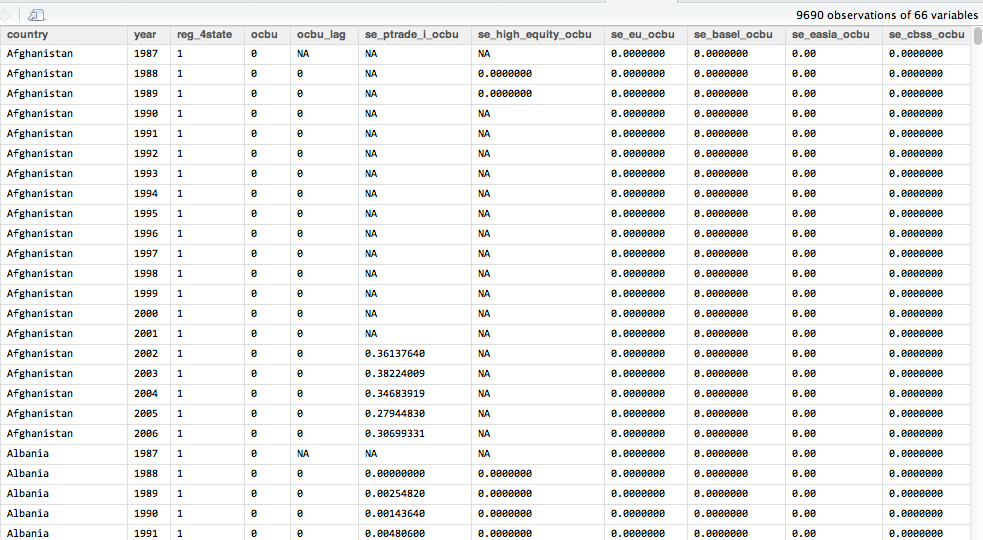
\includegraphics[scale=0.45]{ExampleDataFrameFin.png}
  \end{center}
}

\frame{
  \frametitle{Observations}
  {\LARGE{Observations}} \\[0.5cm]
  Each time we measure our variables we create an {\bf{observation}}, \\[0.5cm]
  {\bf{Observations}} are usually the {\bf{rows}} of the data set. 
}

\frame[plain]{
  \begin{center}
    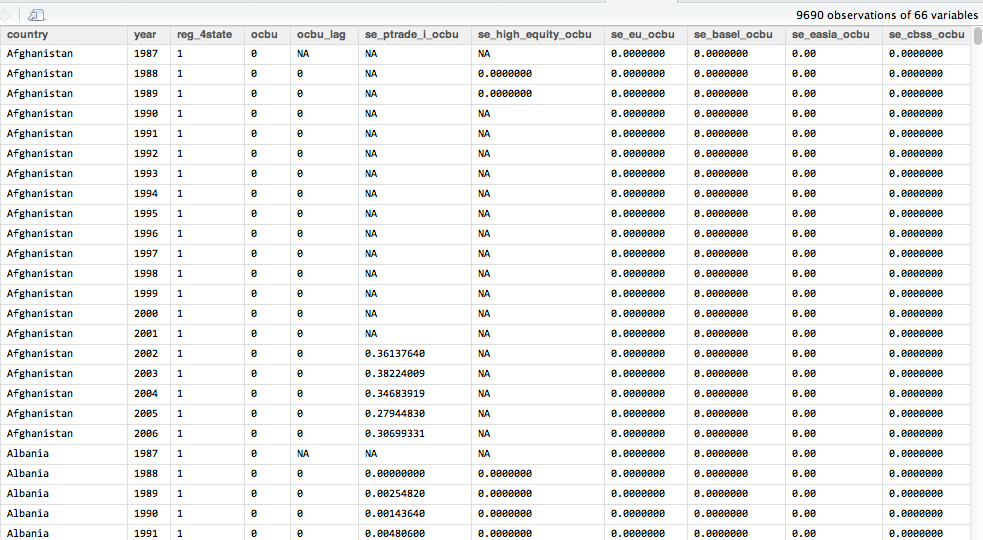
\includegraphics[scale=0.45]{ExampleDataFrameFin.png}
  \end{center}
}

\frame{
  \frametitle{Levels of Measurement}
  Variables can be at different {\bf{levels of measurement}}. \\[0.5cm]
  \begin{center}
    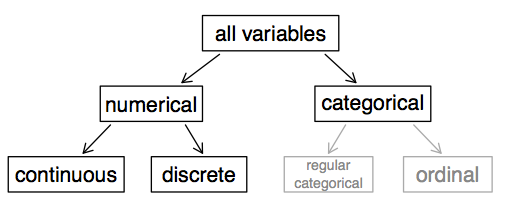
\includegraphics[scale=0.5]{LevelsOfMeasurement.png} \\[0.5cm]
    Source: Diez et al. (2011, 5)
  \end{center}
}

\frame{
  \frametitle{Levels of Measurment Examples}
  \begin{small}
  \begin{table}
    \begin{tabular}{l l p{2cm} p{2cm}}
    \hline
    & & Also Known As & Example \\ 
    \hline \hline
    Numerical & Continuous & & GDP/Capita \\[0.25cm]
     & Discrete & & People in a city \\[0.25cm]
    \hline
    Categorical & Ordinal & & Satisfaction with democracy (5-point scale)\\[0.25cm]
     & Binary & Dummy (0/1) & Gender \\[0.25cm]
     & Nominal & Regular Categorical & Country names 
    \end{tabular}
  \end{table}
  \end{small}
}

\frame{
  \frametitle{Levels of Measurement}
  Levels of measurement are important because they {\bf{determine}} what kinds of {\bf{statistical analyses}} we can do. \\[0.25cm]
  We'll talk more about this beginning Week 5. \\[0.5cm]
  {\bf{Now:}} We need to keep in mind what level of measurement our data is in. \\[0.5cm]
  {\bf{Tip:}} Try to have your data as close to {\bf{Continuous}} as possible.
}

\section{Data Frames in R}
\begin{frame}[fragile]
  \frametitle{Data Frames 1}
  The main type of object we will use in R to store data are called {\bf{data frames}}. \\[0.25cm]
  So far we have worked with matrices.\\[0.25cm]
  Matrices have rows and columns.
\end{frame}

\begin{frame}[fragile]
\begin{knitrout}
\definecolor{shadecolor}{rgb}{0.969, 0.969, 0.969}\color{fgcolor}\begin{kframe}
\begin{alltt}
\hlcomment{# A quick matrix example}
Population <- \hlfunctioncall{c}(14.3, 6.3, 66.7)

Countries <- \hlfunctioncall{c}(\hlstring{"Cambodia"}, \hlstring{"Laos"}, \hlstring{"Thailand"})

NewData <- \hlfunctioncall{cbind}(Countries, Population)

NewData
\end{alltt}
\begin{verbatim}
##      Countries  Population
## [1,] "Cambodia" "14.3"    
## [2,] "Laos"     "6.3"     
## [3,] "Thailand" "66.7"
\end{verbatim}
\end{kframe}
\end{knitrout}

\end{frame}


\begin{frame}[fragile]
  \frametitle{Matrices vs. Data Frames}
  Matrices can only have data with {\bf{one mode}}. \\[0.5cm]
  Data frames can have {\bf{multiple modes}}.\\[0.5cm]
  To create a data frame from multiple vectors use the \texttt{data.frame} command.
\end{frame}

\begin{frame}[fragile]
\begin{knitrout}
\definecolor{shadecolor}{rgb}{0.969, 0.969, 0.969}\color{fgcolor}\begin{kframe}
\begin{alltt}
\hlcomment{# A quick data.frame example}

NewData <- \hlfunctioncall{data.frame}(Countries, Population)

NewData
\end{alltt}
\begin{verbatim}
##   Countries Population
## 1  Cambodia       14.3
## 2      Laos        6.3
## 3  Thailand       66.7
\end{verbatim}
\end{kframe}
\end{knitrout}

\end{frame}

\begin{frame}[fragile]
  \frametitle{Multi-mode data frames}
\begin{knitrout}
\definecolor{shadecolor}{rgb}{0.969, 0.969, 0.969}\color{fgcolor}\begin{kframe}
\begin{alltt}
\hlcomment{# Check variables' class}
\hlfunctioncall{class}(NewData$Countries)
\end{alltt}
\begin{verbatim}
## [1] "factor"
\end{verbatim}
\begin{alltt}

\hlfunctioncall{class}(NewData$Population)
\end{alltt}
\begin{verbatim}
## [1] "numeric"
\end{verbatim}
\end{kframe}
\end{knitrout}

\end{frame}

\frame{
  \frametitle{New Things}
  \begin{itemize}
    \item<1-> What is the dollar sign (\texttt{\$})?
    \item<2-> What is a \texttt{factor}?
  \end{itemize}
}

\frame{
  {\LARGE{Factors 1}} \\[1cm]
  Factors are an R term for {\bf{categorical}} variables.
}

\begin{frame}[fragile]
  \frametitle{Component selector}
  In R the \texttt{\$} is called the {\bf{component selector}}. \\[0.5cm]
  It allows us to {\bf{select a specific column}} of a data set.\\[0.5cm]
\begin{knitrout}
\definecolor{shadecolor}{rgb}{0.969, 0.969, 0.969}\color{fgcolor}\begin{kframe}
\begin{alltt}
\hlcomment{# Select the Countries variable from NewData}
NewData$Countries
\end{alltt}
\begin{verbatim}
## [1] Cambodia Laos     Thailand
## Levels: Cambodia Laos Thailand
\end{verbatim}
\end{kframe}
\end{knitrout}

\end{frame}

\begin{frame}[fragile]
  \frametitle{Factors 2}
  We now have the \texttt{Countries} variable and can see its \texttt{Levels} \\[1cm]
  Giving this variable \texttt{Levels} doesn't really make sense. \\[0.5cm]
  One solustion is to use the \texttt{stringsAsFactors = FALSE} option with \texttt{data.frame}.
\end{frame}

\begin{frame}[fragile]
\begin{knitrout}
\definecolor{shadecolor}{rgb}{0.969, 0.969, 0.969}\color{fgcolor}\begin{kframe}
\begin{alltt}
\hlcomment{# Create data.frame with no factors}
NewData <- \hlfunctioncall{data.frame}(Countries, 
                      Population, 
                      \hlfunctioncall{options}(
                        stringsAsFactors = FALSE))

NewData$Countries
\end{alltt}
\begin{verbatim}
## [1] "Cambodia" "Laos"     "Thailand"
\end{verbatim}
\begin{alltt}

\hlcomment{# Show NewData variable names}
\hlfunctioncall{names}(NewData)
\end{alltt}
\begin{verbatim}
## [1] "Countries"        "Population"      
## [3] "stringsAsFactors"
\end{verbatim}
\end{kframe}
\end{knitrout}

\end{frame}

\begin{frame}[fragile]
  \frametitle{Subsetting 1}
  How do we get rid of the \texttt{StringsAsFactors} variable? \\[0.5cm]
  Use subscripts to {\bf{subset}} the data! \\[0.25cm]
  These are the square braces: \texttt{[]}. \\[0.5cm]
  All cells in an object have an {\bf{address}}: \texttt{[row, column]}. 
\end{frame}

\begin{frame}[fragile]
  \frametitle{Subsetting 2}
  We want to keep the first and second columns and remove the \texttt{StringsAsFactors} variable:
\begin{knitrout}
\definecolor{shadecolor}{rgb}{0.969, 0.969, 0.969}\color{fgcolor}\begin{kframe}
\begin{alltt}
\hlcomment{# Subset NewData, columns 1 & 2}
NewData <- NewData[, 1:2]

\hlcomment{# Show variable names}
\hlfunctioncall{names}(NewData)
\end{alltt}
\begin{verbatim}
## [1] "Countries"  "Population"
\end{verbatim}
\end{kframe}
\end{knitrout}

\end{frame}

\begin{frame}[fragile]
  We'll play around with subscripts a lot more in the seminar. \\[0.25cm]
\end{frame}

\begin{frame}[fragile]
  \frametitle{Subsetting Preview}
  {\bf{Preview:}} We can subset not just by location but also by {\bf{observation value}}.\\[0.25cm]
  For example, to subset the data to include only countries with populations greater than 7 million:
\begin{knitrout}
\definecolor{shadecolor}{rgb}{0.969, 0.969, 0.969}\color{fgcolor}\begin{kframe}
\begin{alltt}
\hlcomment{# Create new object for countries with > 7m pop.}
MoreThan7 <- NewData[NewData$Population > 7, ]

\hlcomment{# Show contents of MoreThan7}
MoreThan7
\end{alltt}
\begin{verbatim}
##   Countries Population
## 1  Cambodia       14.3
## 3  Thailand       66.7
\end{verbatim}
\end{kframe}
\end{knitrout}

\end{frame}

\begin{frame}[fragile]
  Before the seminar it might be a good idea to look at the help file for the \texttt{subset} command.
\begin{knitrout}
\definecolor{shadecolor}{rgb}{0.969, 0.969, 0.969}\color{fgcolor}\begin{kframe}
\begin{alltt}
?subset
\end{alltt}
\end{kframe}
\end{knitrout}

\end{frame}

\begin{frame}[fragile]
  \frametitle{Factor Level Assignment 1}
  What if we have a variable without factor levels, but want to assign them?
\end{frame}

\begin{frame}[fragile]
  \frametitle{Factor Level Assignment 2}
  \begin{small}
  \begin{table}
    \begin{tabular}{l c}
    \hline
    Level & Code \\
    \hline \hline
    Coastal & 1 \\
    Not Coastal & 0
    \end{tabular}
  \end{table}
  \end{small}
\end{frame}

\begin{frame}[fragile]
\begin{knitrout}
\definecolor{shadecolor}{rgb}{0.969, 0.969, 0.969}\color{fgcolor}\begin{kframe}
\begin{alltt}
\hlcomment{# Create variable}
Coastal <- \hlfunctioncall{c}(1, 0, 1)

\hlcomment{# Combine with Countries}
CoastalDF <- \hlfunctioncall{data.frame}(Countries,
                        Coastal,
                        \hlfunctioncall{options}(
                          stringsAsFactors = FALSE))

\hlcomment{# Remove stringsAsFactors variable}
CoastalDF <- CoastalDF[, 1:2]
\end{alltt}
\end{kframe}
\end{knitrout}

\end{frame}

\begin{frame}[fragile]
\begin{knitrout}
\definecolor{shadecolor}{rgb}{0.969, 0.969, 0.969}\color{fgcolor}\begin{kframe}
\begin{alltt}
\hlcomment{# Merge with NewData}
MergedData <- \hlfunctioncall{merge}(x = NewData, 
                    y = CoastalDF, 
                    by = \hlstring{"Countries"})

\hlcomment{# Show variable names}
\hlfunctioncall{names}(MergedData)
\end{alltt}
\begin{verbatim}
## [1] "Countries"  "Population" "Coastal"
\end{verbatim}
\begin{alltt}

\hlcomment{# Show the Coastal variables class}
\hlfunctioncall{class}(MergedData$Coastal)
\end{alltt}
\begin{verbatim}
## [1] "numeric"
\end{verbatim}
\end{kframe}
\end{knitrout}

\end{frame}

\begin{frame}[fragile]
  \frametitle{Factor Level Assignment 3}
  Use the \texttt{factor} command to add the factor levels
\begin{knitrout}
\definecolor{shadecolor}{rgb}{0.969, 0.969, 0.969}\color{fgcolor}\begin{kframe}
\begin{alltt}
\hlcomment{# Turn Coastal into a factor & specify levels}
MergedData$Coastal <- \hlfunctioncall{factor}(MergedData$Coastal,
                                labels = \hlfunctioncall{c}(
                                  \hlstring{"Not Coastal"},
                                  \hlstring{"Coastal"}))

\hlcomment{# Show levels}
MergedData$Coastal
\end{alltt}
\begin{verbatim}
## [1] Coastal     Not Coastal Coastal    
## Levels: Not Coastal Coastal
\end{verbatim}
\end{kframe}
\end{knitrout}

  
\end{frame}

\begin{frame}[fragile]
  \frametitle{Merging 1}
  What was this?
\begin{knitrout}
\definecolor{shadecolor}{rgb}{0.969, 0.969, 0.969}\color{fgcolor}\begin{kframe}
\begin{alltt}
\hlcomment{# Merge with NewData}
MergedData <- \hlfunctioncall{merge}(x = NewData, 
                    y = CoastalDF, 
                    by = \hlstring{"Countries"})
\end{alltt}
\end{kframe}
\end{knitrout}

\end{frame}

\begin{frame}[fragile]
  \frametitle{Merging 2}
  We saw how you can use the \texttt{cbind} command to attach columns together. \\[0.5cm]
  This is usually {\bf{not}} a good way to merge two data sets together. \\[0.5cm]
  For \texttt{cbind} the observations have to be in the {\bf{same order}} in both objects. \\[0.5cm]
  This is {\bf{very uncommon}}.
\end{frame}

\begin{frame}[fragile]
  \frametitle{Merging 2}
  The \texttt{merge} command matches each observation.\\[0.5cm]
  You tell it what the {\bf{observation ID variable}} is with the \texttt{by} argument.\\[0.25cm]
  For example \texttt{by = "Countries"} \\[0.5cm]
  We'll see more of this next week.
\end{frame}


\section{First Assignment}
\frame{
  \frametitle{First Assignment}
  {\large{{\bf{Due:}} Monday 24 September}} \\[0.5cm]
  Create a new data frame with country-level data from at least {\bf{two}} different sources. \\[0.5cm]
  Create a folder in your Dropbox \texttt{Public} folder and {\bf{email me the link}}. \\[0.5cm]
  The folder needs to include:
  \begin{enumerate}
    \item<1-> The new data frame saved as a \texttt{.csv} file.
    \item<1-> A text file {\bf{describing the variables and their sources}}.
    \item<1-> A notebook \texttt{.html} file detailing how you created the data frame and saved it as a\texttt{.csv}.
  \end{enumerate}
}

\begin{frame}[allowframebreaks]
  \frametitle{References}
  Diez, David M., Christopher D. Barr, and Mine \c{C}etinkaya-Rundel. OpenIntro Statistics. 1st ed. \url{http://www.openintro.org/stat/downloads.php}. \\[0.25cm] 
  
  Weeks, Jessica L. 2012. “Strongmen and Straw Men: Authoritarian Regimes and the Initiation of International Conflict.” American Political Science Review 106(2): 326–347.
\end{frame}

\end{document}
